\chapter{REAL-TIME PARTICLE SYSTEMS LIBRARY}\label{RTPSchapter}

% Introduction
%\section{Introduction}
The Real-Time Particle Systems (RTPS) library was designed and developed by Ian Johnson\cite{ianPaper}, including a particle module. In this thesis, we have extended RTPS to include a flocking (boid) system. 

This chapter introduces the RTPS framework. The description of the RTPS library follows the structure of the RTPS implementation showed in Figure~\ref{RTPSdiagram}. At the end of the Chapter, we provide a detailed description of the extended implementation developed for the \texttt{FLOCK} system.

% RTPS diagram
\begin{figure}[htbp]
\begin{center}
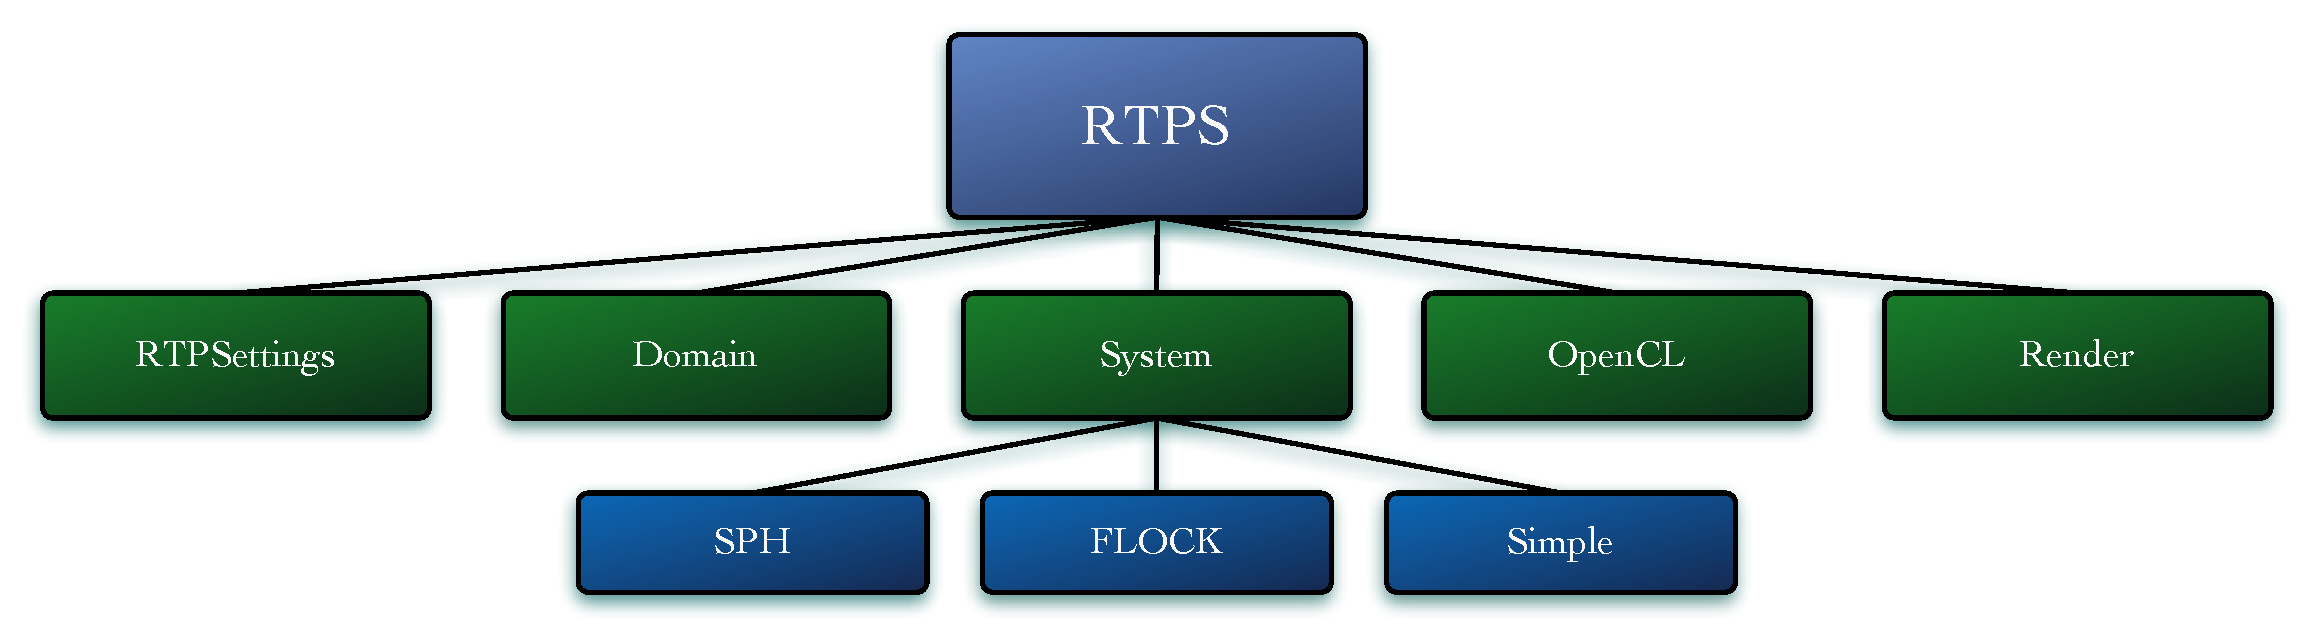
\includegraphics[scale=0.38]{figures/RTPSdiagramMyrna.pdf}
\caption{RTPS hierarchy diagram: depicts the structure of the RTPS library}
\label{RTPSdiagram}
\end{center}
\end{figure}

% RTPS
\section{RTPS}\label{rtpssection}
\texttt{RTPS.h} is the main class of the RTPS library. An \texttt{RTPS} object is a particle system initialized with a set of user settings,  discussed in Section~\ref{rtpsettings}. 

As seen in Figure~\ref{RTPSdiagram}, \texttt{RTPS} is the root of the library. Only two methods are defined in the \texttt{RTPS} class: \texttt{update()} and \texttt{render()}. \texttt{update()} computes the positions of the particles at each frame, and \texttt{render()} is in charge of rendering the particles. These methods are implemented individually by each of the systems available in the RTPS library. The following code shows the \texttt{RTPS} constructor used when creating the \texttt{FLOCK} system.

%\texttt{RTPS} has various instance variables: a \texttt{CL} object which is used to manage the \textit{OpenCL} functionality,  an \texttt{RTPSettings} object to manage the settings of the system and a \texttt{System} object which stores the type of particle system that has been created. 
% RTPS constructor

\begin{cppcode}{0}
RTPS::RTPS(RTPSettings *s, CL* _cli) 
{
	cli = _cli;
 	cl_managed = false;
	settings = s;
	Init();
}
\end{cppcode}

The \texttt{Init()} method called inside the constructor would creates the respective particle system, i.e. \texttt{SPH} or \texttt{FLOCK}, depending on the settings.

% RTPSettings
\section{RTPS Settings}\label{rtpsettings}
\texttt{RTPSettings} is the class that stores all the settings of the particle systems. This class defines the set of systems available in RTPS. The settings are defined depending on the systems. Two systems are currently available SPH and FLOCK. The constructor used to create the RTPS settings is presented below. \texttt{Systype} is an enumeration with the names of the two systems. 

%The location of this class is at \texttt{rtpslib/RTPSettings.h}. It has the following instance variables defined: the maximum number of particles, the time step, and a \texttt{Domain} object. Also, there is an enumeration variable \texttt{SysType} that defines the names of the three available particle systems. Some of the rendering settings are set and get in this class. Here is the \texttt{RTPSettings} constructor that we use for the \texttt{FLOCK} system.

% RTPSettings constructor
\begin{cppcode}{0}
RTPSettings::RTPSettings(SysType system, int max_particles, float dt, Domain* grid)
{
	changed = false;
	this->system = system;
	this->max_particles = nlpo2(max_particles);
	this->dt = dt;
	this->grid = grid;
}
\end{cppcode}

%The parameters for this constructor are the type of system, the maximum number of particles, the time step and the grid domain. 
As an OpenCL requirement, the maximum number of particles has to be a power of two. 

% Domain
\section{Domain}
The \texttt{Domain} class defines the grid in which the simulation is being computed. This class also stores the different grid parameters that are needed throughout the computation. The \texttt{IV} class defines and implements the methods that initialize the positions of the particles. Various geometric shapes are available to initialize the positions: rectangles, spheres, and discs. The \texttt{UniformGrid} class is used in the nearest neighbor search.

% Render
\section{Render}
Most of the code developed for rendering within the RTPS library was developed by Andrew Young\cite{andrewBlog}. There are several of possible rendering choices. The \texttt{Render} type renders the particles as Points; the \texttt{SpriteRender} uses a 2D image and mapped into a sphere and represents each particle as a textured sphere. \texttt{SSFRender} was specifically designed for the SPH system to provide a more "fluid-like" character to the flow. Finally, \texttt{Sphere3DRender} renders the boids as 3D spheres.  

% System
\section{System}
Each of the particle systems in the RTPS library inherits the \texttt{System} class, which contains virtual functions that are shared by the two systems. These functions are related to the rendering,  the domain, and to other shared classes. 

% Common
\section{Common}\label{commonsection}
The RTPS library has shared classes that are used for all systems. These classes share the implementation of a hose, used to spray particles into the physical domain. The other common classes include classes for the nearest neighbor search. The next section explains the nearest neighbor search algorithm.

% NNS
\subsection{Nearest Neighbor Search}
The nearest neighbor search consists of two phases: \textit{preparation} and \textit{lookup}. The following following steps explain how the \textit{preparation} phase is accomplished.

% preparation
\begin{enumerate}
\item{\textbf{Hash}: creates a hash value by overlaying a uniform grid on the system's domain, and calculating an index value from the 3D cell index. Each boid lies in one cell and has an associated hash.}
\item{\textbf{Sort}: sorts the hash array with respect to hash, imposing an ordering on the particles. All particles in a given cell are contiguous in the sorted particle array.}
\item{\textbf{Permute}:  permutes the arrays of positions, velocities, and color according to the sorted index array}
\item{\textbf{Cell indices}: updates two arrays: \texttt{cell\_indices\_start} and \texttt{cell\_indices\_end} that keep track of which cells are populated with particles, \texttt{cell\_indices\_start} stores the index of the first particle in each cell, when there is no particle an index of $-1$ is assigned; the \texttt{cell\_indices\_end} arrays stores the index of the last particle in that cell}
\end{enumerate}

Once the preparation is complete, neighbor search is straightforward and consists of the following three functions:  

% lookup
\begin{enumerate}
\item{\textbf{IterateParticleInNearbyCells}: loops over the 26 cells surrounding the cell of the particle in question. This function calls \texttt{IterateParticlesInCells} for each cell }
\item{\textbf{IterateParticlesInCells}: loops over the particles from the starting to the ending indices of that cell and calls \texttt{ForNeighbor} for each particle}
\item{\textbf{ForNeighbor}: has access to both the particle and its neighbor, from which the influence of a single boid on the steering velocity can be computed.}
\end{enumerate}

The three main steering behaviors use the nearest neighbor search to compute the respective rules in the local neighborhood of each boid.

% SPH
\section{SPH}\label{sphsection}
\texttt{SPH} is the main system of the RTPS library. This system uses the SPH formulation to compute the different forces between particles.

Both the \texttt{FLOCK} and \texttt{SPH} systems are particle-based and depend on a neighbor search to determine either velocities or forces. In the SPH formulation particle-particle interactions generated forces, while in the FLOCK formulation boid-boid interaction generates velocity 
vectors that steer the boids. Both boids and fluid particles are integrated over time to update particle positions.

For more detailed information about the \texttt{SPH} system implemented in the RTPS library, please refer to the Master thesis of Ian Johnson \cite{ianThesis}.

% FLOCK
\section{FLOCK}\label{flocksection}
The \texttt{SPH} system served as a guide to create the \texttt{FLOCK} system with the root class \texttt{FLOCK}. The settings of the \texttt{FLOCK} system are stored in the \texttt{FLOCKSettings} class. 

We implemented the three main steering behaviors of flocking, in addition to the goal and avoid behaviors. Figure~\ref{flockdiagram} shows the hierarchy of the \texttt{FLOCK} system. Most of the classes are detailed in this Section. 

% FLOCK diagram
\begin{figure}[htbp]
\begin{center}
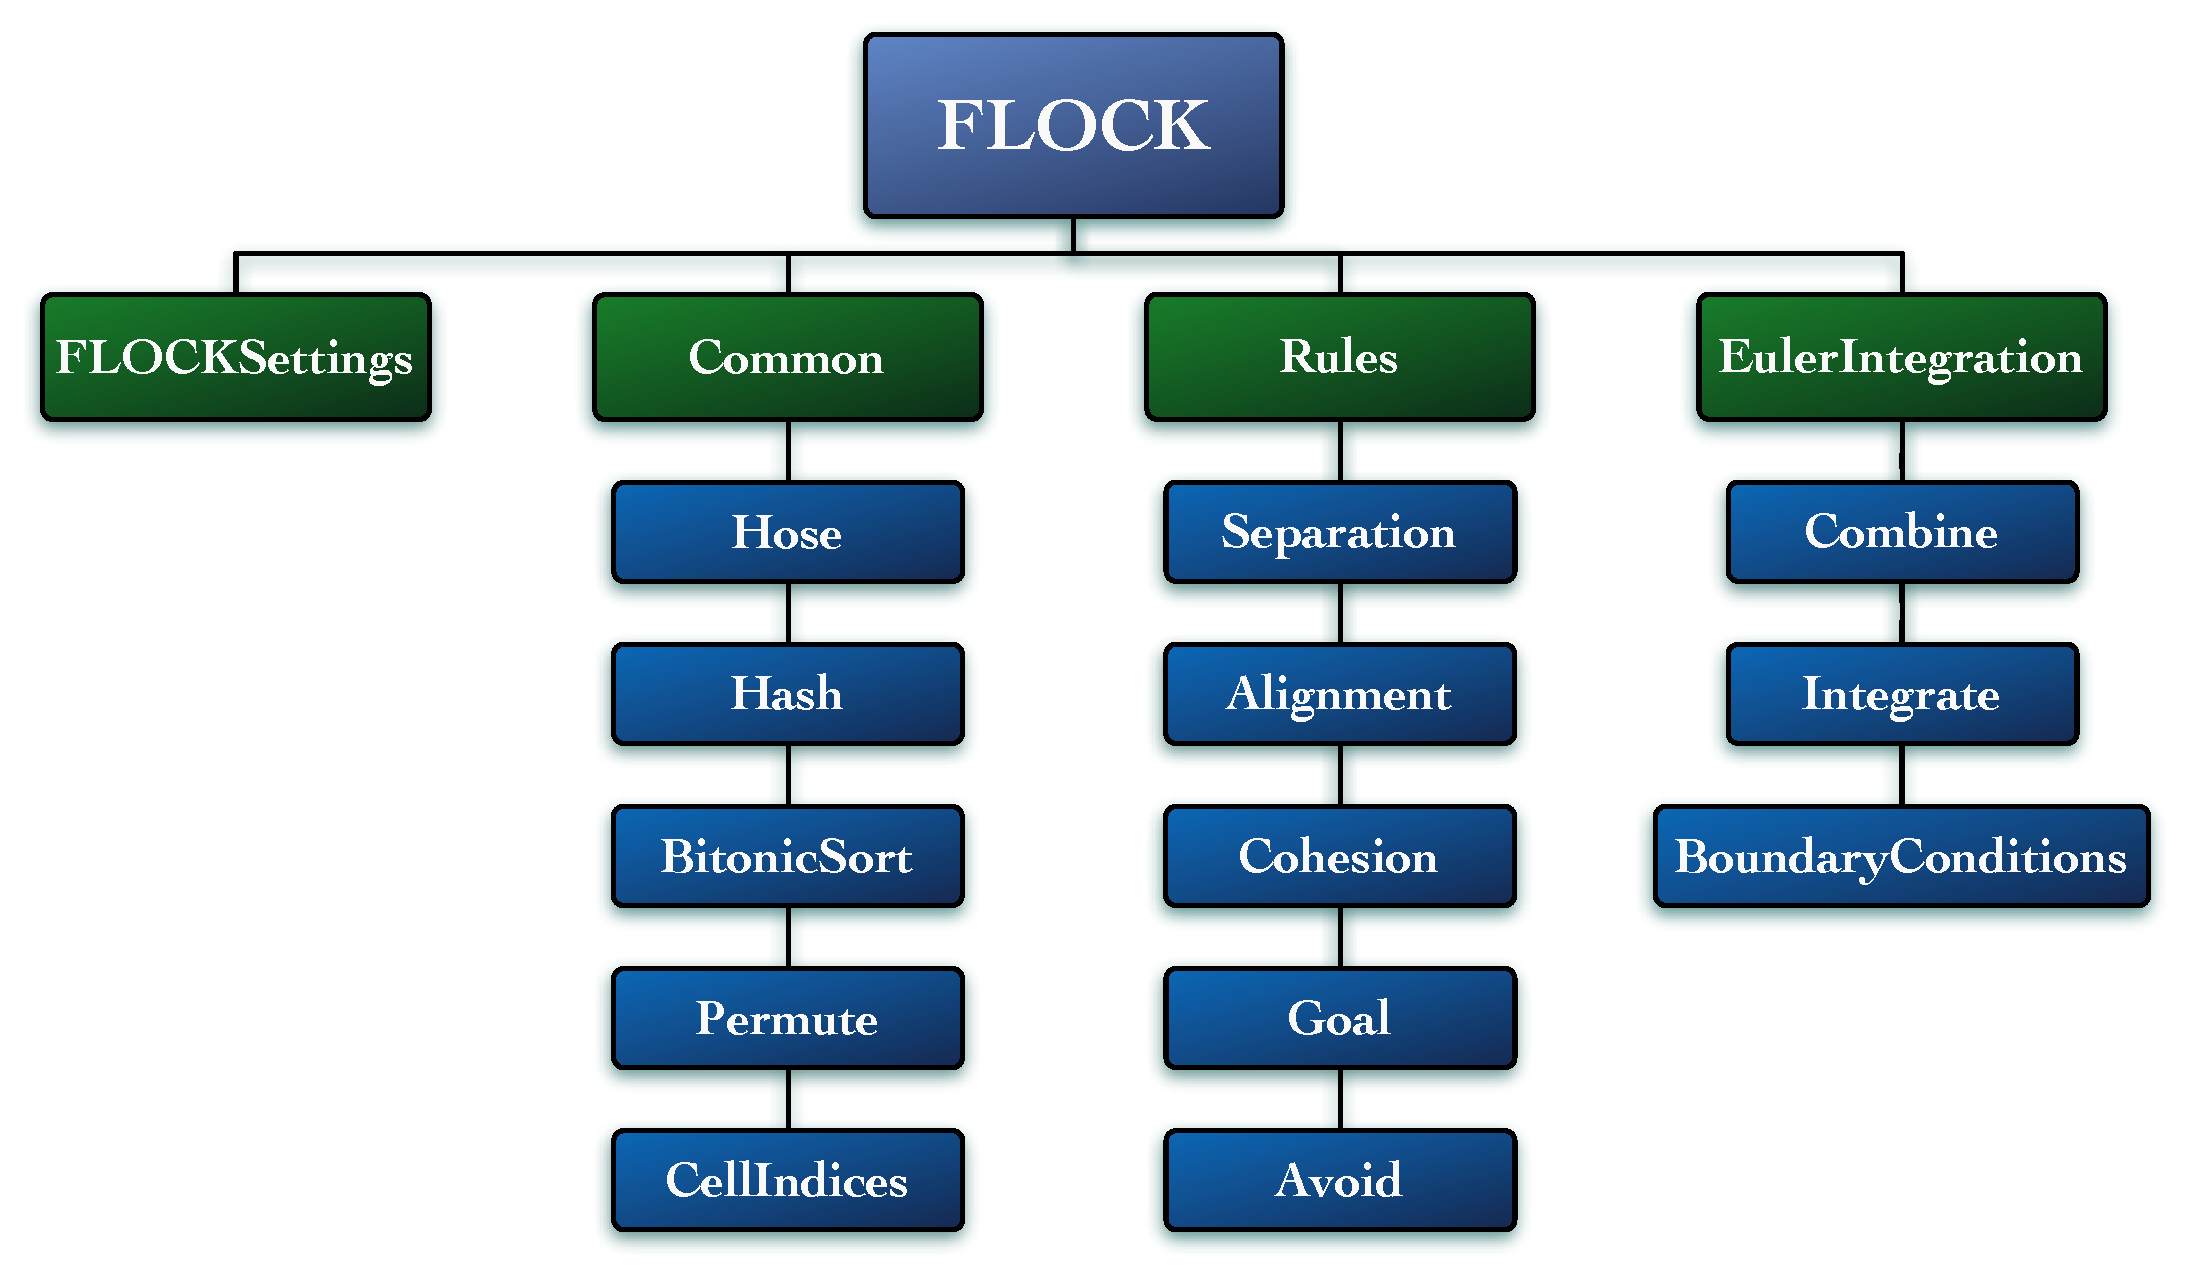
\includegraphics[scale=0.42]{figures/FLOCKdiagramMyrna.pdf}
\caption{FLOCK class hierarchy diagram.} 
\old{depicts the hierarchy of the classes developed for the FLOCK system}
\label{flockdiagram}
\end{center}
\end{figure}


% FLOCK class
\subsection{FLOCK class}
The header file of the \texttt{FLOCK} class defines the prototypes of the functions used to insert particles into our system. It is used to stored all vectors and buffers related to the boids. The following code illustrates the class constructor. 

\begin{cppcode}{0}
FLOCK::FLOCK(RTPS *psfr, int n)
 {
 	//store the particle system framework
 	ps = psfr;
	settings = ps->settings;
	grid = settings->grid;
	max_num = n;
	
	// initial number of particles
	num = 0;
 	
	...
 
 	// calculate and update the parameters
	calculate();
	updateFLOCKP();

	...

	//set up the grid
	setupDomain();
	
	//setup the sorted and unsorted arrays
	prepareSorted();
 	 
	 ...
		
	// create the renderer object depending on the render type		
	setRenderer(); 
}
\end{cppcode}

First, some of the instance variables are initialized. The settings of \texttt{FLOCK} are stored in a structure called \texttt{FLOCKParameters}. When executing \texttt{calculate()}, the parameters 
are set to their default values. Then, \texttt{updateFLOCKP()} updates the parameters to the user settings.

The function \texttt{prepareSorted()} initializes the different vectors and buffers that were created for our system, i.e \texttt{velocities}, \texttt{flockmates}, etc. This function also creates the Vertex Buffer Objects (VBOs). VBO objects store vertex data meant to be used during the rendering process {\em its aim to be used for rendering purposes}\cite{vbo}. Their use makes it possible for the vertex data to be a part of the GPU boid kernels, and of the rendering process without additional data copies or data transfers to and from the CPU. The positions and color vectors are then copied to the respective VBOs. If using the GPU the different \texttt{Buffer} objects are initialized with their respective CPU arrays. The \texttt{FLOCK} parameters are also copied to the GPU. 

\subsubsection{Particles insertion}
The system has being created and now the question arise in \textit{how do the particles are inserted into the system?} There are a few functions defined in the \texttt{FLOCK} that do that task. These functions are \texttt{addBox} , \texttt{addBall}, and \texttt{addHose}. First, these functions initialize the positions of the particles, then the positions of the particles are send to the GPU or CPU to be rendered. 

\subsubsection{Update}
As mentioned in Section~\ref{rtpssection}, each of the systems implements the methods \texttt{update()} and \texttt{render()}. In \texttt{FLOCK} the \texttt{update()} function updates the positions of the boids at each iteration (one iteration per frame). In the CPU implementation, \texttt{updateCPU()} function is called. In turn, this function calls the functions \texttt{cpuRules()} and \texttt{cpuEulerIntegration()}, responsible for the boid position update on the CPU. The CPU code was developed for testing and debugging purposes only. On the other hand, on the GPU, one uses the functipn \texttt{updateGPU()}, which calls the OpenCL kernels that perform the nearest neighbor search, then computes the flocking rules, and finally updates the boid positions. These kernels are described in more detail in Section~\ref{rulesclass}.

% FLOCKSettings class
\subsection{FLOCKSettings class}
In order to run a simulation, the settings of the system need to be set. The specific settings that related to flocking are defined in class \texttt{FLOCKSettings}. The \texttt{FLOCKParameters} struct stores all these settings. This struct includes variables such as the simulation scale, the searching radius, the maximum speed of the boids and the weights of each of the 
steering behaviors. 

% Rules class
\subsection{Rules class}\label{rulesclass}
The \texttt{Rules} class computes the different steering behaviors that were implemented to simulate the flocking behavior. The steering behaviors or \textit{rules} are implemented both on the CPU and on the GPU. All the rules that run on the GPU are computed in the \texttt{rules} kernel. The following code shows the class \texttt{Rules}.

\begin{cppcode}{0}
#ifndef RTPS_RULES_H_INCLUDED
#define RTPS_RULES_H_INCLUDED

#include <CLL.h>
 #include <Buffer.h>

namespace rtps
 {
	class Rules
	{
		public:
			// constructors
			Rules() { cli = NULL; timer = NULL; };
			Rules(std::string path, CL* cli, EB::Timer* timer);
			
			// execution of kernels
			void execute( /* arguments */ );
			
		private:
			// OpenCL
			CL* cli;
			
			// kernels
			Kernel k_rules;
			
			// timer
			EB::Timer* timer;
	};
}
#endif
\end{cppcode}

First, the kernel is initialized in the constructor of class \texttt{Rules}. The kernel 
arguments are set in the \texttt{execute()} method of this class. 

The next code is part of the \texttt{Rules.cpp} file.

\begin{cppcode}{0}
#include<FLOCK.h>
#include<math.h>

namespace rtps
{
	// Rules constructor
	Rules::Rules(std::string wpath, CL* cli_, EB::Timer* timer_)
	{
		...
		try
		{
			path = wpath + "/rules.cl";
			k_rules = Kernel(cli, path, "rules");
		}
		....
	}

	void Rules::execute( /* arguments */ )
	{
		// set the arguments for the kernel
		int iarg = 0;
		k_rules.setArg(iarg++, pos_s.getDevicePtr());
		k_rules.setArg(iarg++, vel_s.getDevicePtr());
		...
	}
	...
	
	void FLOCK::cpuRules()
	{
		...
	}
}
\end{cppcode}

The implementation of the kernel is stored separately from the c++ classes in order to better 
modularize our framework. 
\old{better distinguish between the C++ and the OpenCL files.}
The kernel defined in \texttt{Rules} is called \texttt{rules}. 
\old{Each rule was implemented in an individual file that is included where the respective rule is called. }
\old{Those files are \texttt{rule\_separation}, \texttt{rule\_alignment}, \texttt{rule\_cohesion}, \texttt{rule\_goal}, and \texttt{rule\_avoid}. The \texttt{rules} kernel implements the Algorithm~\ref{flockingAlgorithm}.}

%, and \texttt{rule\_leaderfollowing}.

%\texttt{\textbf{flockmates}} looks for the neighbors and determines which ones are within the searching radius, and count them. Also, it counts how many neighbors are within the minimum separation distance of each boid. At the end, the vector \texttt{flockmates} which was allocated in the GPU is updated with the values obtained.

%\texttt{\textbf{rule\_separation}} is computed using the neighbors that are within the minimum separation distance\footnote{for more details on how the rule is computed see the formulation of Separation in Section~\ref{separationsection}}. The behavior is accumulated in a vector. After the neighbors within the minimum distance are processed, the behavior vector is averaged over the number of flockmates found within the minimum separation distance, then the vector is normalized. Finally, the value of the vector \texttt{separation} are copied to the vector allocated in the GPU.

%\texttt{\textbf{rule\_alignment}} determines which neighbors are within a prescribed radius, the velocities of those neighbors are accumulated. Then, the average is taken using the number of flockmates following by a subtraction of the average velocity and the boids velocity. At the end the vector obtained is used to update the respective vector in the GPU. 

%\texttt{\textbf{rule\_cohesion}} is analogous to the alignment rule, the only difference is that positions are used instead of velocities.

%\texttt{\textbf{rule\_leaderfollowing}} \textcolor{red}{*** TODO: still need to develop the leader behavior, then I would write the description of this kernel ***}

%This would finish the description of the \texttt{Rules} class. The next step is to integrate over time to get the new position of the boid.

% Euler Integration class
\subsection{EulerIntegration class}
%A discussion on how to get the different steering behaviors vectors have been done. 
This Section describes briefly how to combine the vectors that stores the behaviors in order to get one single vector to update the positions. A class called \texttt{EulerIntegration} was developed in order to get the new positions. The {EulerIntegration.h} class is shown bellow.

\begin{cppcode}{0}
#ifndef RTPS_EULER_INTEGRATION_H_
#define RTPS_EULER_INTEGRATION_H_

#include <CLL.h>
#include <Buffer.h>

namespace rtps
{
	class EulerIntegration
	{
		public:
			EulerIntegration() { cli = NULL; timer = NULL; };
	 		EulerIntegration(std::string path, CL* cli, EB::Timer* timer);
			void execute( /* arguments */ );

		private:
			CL* cli;
			Kernel k_euler_integration;
			EB::Timer* timer;
	};
}
#endif
\end{cppcode}

The structure of the \texttt{EulerIntegration} class is similar to that of the \texttt{Rules} class. \texttt{EulerIntegration.cpp} initializes the kernel and implements the \texttt{execute} function that sets the arguments of the kernels and executes it. It also carries the implementation of the function \texttt{cpuEulerIntegration()}. 

The kernel \texttt{\textbf{euler\_integration}} starts by retrieving the respective steering vectors and weights from the GPU.The weights are obtained from the flocking parameters object. The velocity vectors for each of the rules are then computed and combined to obtain the final velocity vector.

\begin{cppcode}{0}
// RULE 1. SEPARATION
vel_sep = separation * w_sep;
   
// RULE 2. ALIGNMENT
vel_aln = alignment * w_aln;

// RULE 3. COHESION
vel_coh = cohesion * w_coh;

// RULE 4. GOAL
vel_goal = goal * w_goal;

// RULE 5. AVOID
vel_avoid = avoid * w_avoid;

// FINAL VELOCITY
vel = vi + vel_sep + vel_aln + vel_coh + vel_goal + vel_avoid;
\end{cppcode}

Finally, the final velocity is constrained to a prescribed maximum speed. As an option, the boids can be subjected to an imposed velocity field, which is added to the steering velocity to obtain the actual vector used to move the boid. Finally, the updated boid positions are computed using the steering velocity.

\begin{cppcode}{0}
// OPTIONAL CIRCULAR VELOCITY FIELD
float4 v = (float4)(-3*pi.z, 0.f , pi.x, 0.f);
v *= flockp->circular_vel_const;

// SET THE NEW VELOCITY
vi = v + acc;
vi.w = 0.f;

// INTEGRATION
pi += dt*vi; 
\end{cppcode}
 


